%
\chapter{Runtime execution}
%


\section{Distributed runtime model}

As it has been stated before, the model of the system is stored distributedly on different computation unit. A model element only stored in a given computation unit. References can occur between elements in different partitions, so we create proxy objects, that represents an object from another partition, and the local object stores reference to that object. For example, on figure~\ref{fig:distrib-model-example} this can be seen. There are three computing units called \texttt{BBB1}, \texttt{BBB2} and \texttt{BBB3}. \texttt{s5}, \texttt{tr1}, \texttt{s4} and \texttt{s3} are located on \texttt{BBB2}. 

\begin{figure}[h]
	\begin{center}
		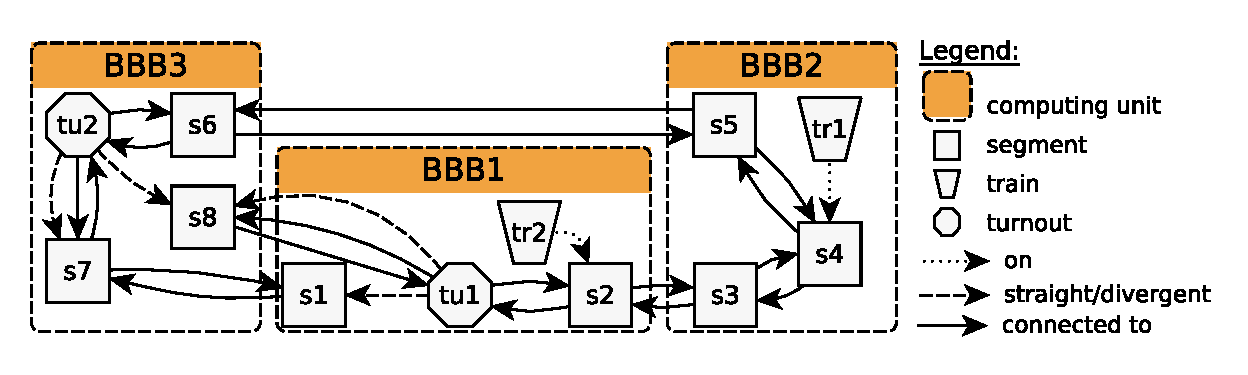
\includegraphics[width=0.9\textwidth]{figures/runtime-snapshot.pdf}
		\caption{Example for a distributed model}
		\label{fig:distrib-model-example}
	\end{center}
\end{figure}




\section{Distributed query execution}


\subsection{Distributed local search}

As models are stored on different computational units we still needs to find matches, that can span over multiple model parts. To find matches for a pattern local search algorithm is used in a distributed way. Search operations are being executed locally, and if the next operation needs to be executed on multiple nodes, the search context, (ie.\ the bound variables and the operations number) are sent to other computational units.

\begin{figure}[h]
	\begin{center}
		\includegraphics[width=1\textwidth]{figures/seq-diagram-query-exec.png}
	\end{center}
\end{figure}
\todo{ábra okosítás}